% !TEX TS-program = pdflatex
% !TEX encoding = UTF-8 Unicode

% This is a simple template for a LaTeX document using the "article" class.
% See "book", "report", "letter" for other types of document.

\documentclass[11pt]{article} % use larger type; default would be 10pt

\usepackage[T1]{fontenc}
\usepackage[utf8]{inputenc} % set input encoding (not needed with XeLaTeX)
\usepackage[ngerman]{babel}
\usepackage{marvosym}
\DeclareUnicodeCharacter{20AC}{\EUR}

%%% Examples of Article customizations
% These packages are optional, depending whether you want the features they provide.
% See the LaTeX Companion or other references for full information.

%%% PAGE DIMENSIONS
\usepackage{geometry} % to change the page dimensions
\geometry{a4paper} % or letterpaper (US) or a5paper or....
% \geometry{margin=2in} % for example, change the margins to 2 inches all round
% \geometry{landscape} % set up the page for landscape
%   read geometry.pdf for detailed page layout information

\usepackage{graphicx} % support the \includegraphics command and options

% \usepackage[parfill]{parskip} % Activate to begin paragraphs with an empty line rather than an indent

%%% PACKAGES
\usepackage{booktabs} % for much better looking tables
\usepackage{array} % for better arrays (eg matrices) in maths
\usepackage{paralist} % very flexible & customisable lists (eg. enumerate/itemize, etc.)
\usepackage{verbatim} % adds environment for commenting out blocks of text & for better verbatim
\usepackage{subfig} % make it possible to include more than one captioned figure/table in a single float
% These packages are all incorporated in the memoir class to one degree or another...

%%% HEADERS & FOOTERS
\usepackage{fancyhdr} % This should be set AFTER setting up the page geometry
\pagestyle{fancy} % options: empty , plain , fancy
\renewcommand{\headrulewidth}{0pt} % customise the layout...
\lhead{}\chead{}\rhead{}
\lfoot{}\cfoot{\thepage}\rfoot{}

%%% SECTION TITLE APPEARANCE
\usepackage{sectsty}
\allsectionsfont{\sffamily\mdseries\upshape} % (See the fntguide.pdf for font help)
% (This matches ConTeXt defaults)

%%% ToC (table of contents) APPEARANCE
\usepackage[nottoc,notlof,notlot]{tocbibind} % Put the bibliography in the ToC
\usepackage[titles,subfigure]{tocloft} % Alter the style of the Table of Contents
\renewcommand{\cftsecfont}{\rmfamily\mdseries\upshape}
\renewcommand{\cftsecpagefont}{\rmfamily\mdseries\upshape} % No bold!

%%% END Article customizations

%%% The "real" document content comes below...

\title{Handbuch „Cash Register“ \\ \large Ein einfaches RFID gestütztes Bezahlsystem mit Datenbankanbindung als geschlossenes System}
\author{Moritz Hilberg 733760 \and Lukas Köhler 734188}
%\date{} % Activate to display a given date or no date (if empty),
         % otherwise the current date is printed 

\begin{document}
\maketitle
~\newline
\newline
\newline
\newline
\newline
\tableofcontents
\newpage
\section{Installation und unterstützte Hardware}
\subsection{Installation und Starten des Programms}
Um das System zu installieren, genügt es, den Ordner
\textit{AbgabeProtokoll/JarExport/} auf das eigene Betriebssystem zu kopieren
und die Datei \textit{CashRegister.jar} zu starten. Diese öffnet dann direkt das
User-Interface des Programms. Wichtig ist, dass eine JRE installiert ist, da
sonst \textit{CashRegister.jar} nicht gestartet werden kann. Weitere genutzte
Bibliotheken wie \textit{jSSC} oder \textit{sqlite3} müssen nicht manuell
installiert werden, da diese bereits im \textit{.jar} Paket liegen und auch dort
referenziert werden.
\subsection{Bibliotheken und Datenbank}
\textit{jSSC} ist für das Lesen und Schreiben einer
seriellen Verbindung und \textit{sqlite3} für das Lesen und Schreiben einer
Datenbank. Die Datenbank für das System befindet sich in dem Ordner
\textit{AbgabeProtokoll/JarExport/database/} und kann bei Bedarf manuell mit
einem Datenbank-Programm wie z.B. dem passenden sqlitebrowser
(\textit{http://sqlitebrowser.org/}) geöffnet und beschrieben werden. Die
Datenbank umfasst alle User mit Namen und einer passenden Tag-ID, um sie später
einem passenden RFID-Tag zuordnen zu können, Transactions, welche alle
getätigten Transaktionen in Bezug auf ein User enthält und Values, welche die
Geldscheine anhand weiterer RFID-Tags simuliert und jeweils einen Betrag und 
eine Tag-ID enthält. 
\subsection{Konfigurationsdatei}
Weiter umfasst das Programm eine Konfigrationsdatei
(\textit{AbgabeProtokoll/JarExport/configFile}), welche die Befehle für die
serielle Schnittstelle enthält. Befehl und zu erwartende Antwort sind durch ein
Semikolon getrennt. Die Datei enthält die Befehle, welche bei Start
des Programms als Setup an die serielle Schnittstelle geschickt werden und die
Befehle die benötigt werden um einen RFID-Tag auszulesen. Die zu erwartende
Antwort wird dabei jeweils mit der zurückgekommenen Antwort verglichen.
\subsection{Betriebssystem}
Das Programm wurde unter Linux entwickelt und getestet, kann jedoch
plattformunabhängig unter jedem Betriebssystem mit einer funktionsfähigen JRE
gestartet werden, da sämtliche Bibliotheken selbst im \textit{.jar} Paket liegen
und diese ebenfalls platformunabhängig sind.
\subsection{Reader-Board}
Um RFID-Tags zu lesen, wurde das \textit{Atmel ATA 2270-EK1} benutzt. Da ein
Bezahlsystem auf keine hohen Reichweiten ausgelegt sein soll, entschieden wir
uns bei dem Vergleich eines LF- beziehungsweise HF-Systems für Ersteres. Auf die
Konfiguration und Installation des \textit{Atmel ATA 2270-EK1} wird hier nun
nicht weiter eingegangen, da dies detailert in Termin 3 des Praktikums
durchgeführt wurde.
\section{Benutzerführung und Funktionen}
Abbildung \ref{snapshot1} zeigt den erfolgreich eingelesenen Tag-ID
\textit{moritzTagID}, welcher im Feld \textit{Customer ID} nochmals
dargestellt ist. Weiterhin ist der Name in dem Feld \textit{Name} und der
aktuelle Kontostand in \textit{Balance} zu sehen. Dieser beträgt in diesem Fall
zurzeit 0. Das grüne Label unten weist hinzukommend auf das erfolgreiche
Einlesen und Erkennen hin. \textit{Counter} zeigt, wie oft derselbe Tag hintereinander
eingelesen wurde, falls dieser sich länger in der Reichweite des Lesegerätes
befindet.
\begin{center}
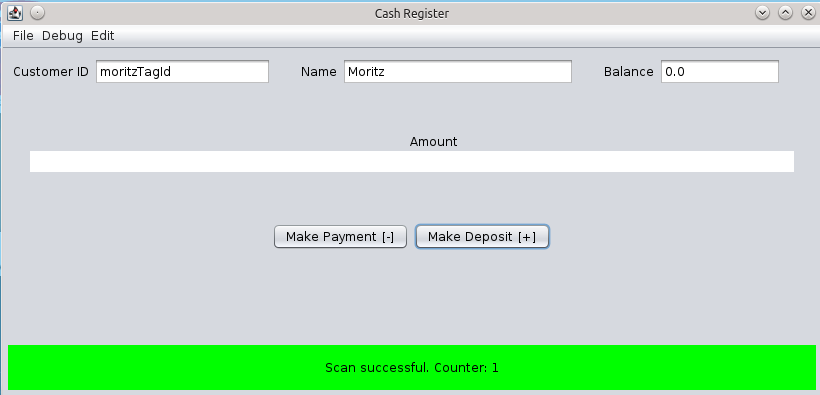
\includegraphics[height=5cm,keepaspectratio]{snapshot1.png}
\captionof{figure}{Tag-ID \textit{moritzTagID} wurde eingelesen}
\label{snapshot1}
\end{center}
~\newline
In Abbildung \ref{snapshot2} wurde um Geld einzuzahlen zuvor auf \textit{Make
Deposit} geklickt. In diesem Beispiel wurden Value-Tags mit 20.0 und 5.0
hintereinander eingelesen. Wie zu sehen ist, werden diese direkt summiert. Wird
die Aktion mit einem Klick auf \textit{Ok} bestätigt, wird die Transaktion
ausgeführt und anschließend in der Datenbank gespeichert.
\begin{center}
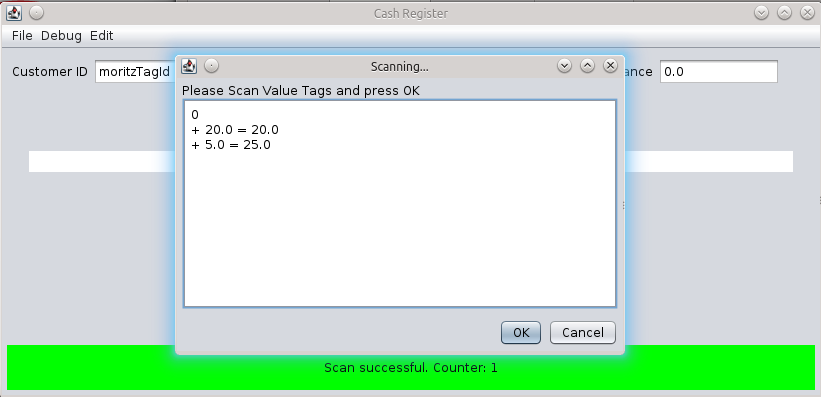
\includegraphics[height=5cm,keepaspectratio]{snapshot2.png}
\captionof{figure}{Make Desposit}
\label{snapshot2}
\end{center}
\begin{center}
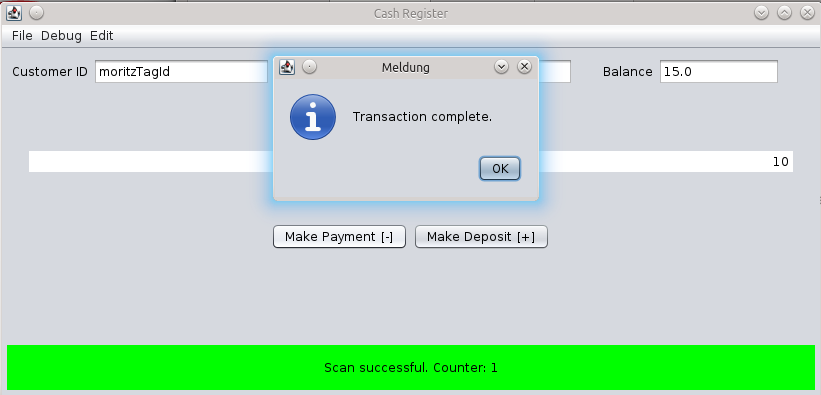
\includegraphics[height=5cm,keepaspectratio]{snapshot3.png}
\captionof{figure}{Make Payment}
\label{snapshot3}
\end{center}
Abbildung \ref{snapshot3} zeigt das Gegenteil zu Abbildung \ref{snapshot2}. Hier
wird nun Geld ausgezahlt, indem der Benutzer seinen gewünschten Betrag in das
Feld \textit{Amount} einträgt und anschließend mit \textit{Make Payment} die
Transaktion bestätigt. Der Betrag wird dann vom Konto abgezogen und in die
Datenbank gespeichert.
\newline
\newline
In Abbildung \ref{snapshot4} wurde ein Tag eingescannt, dessen ID der Datenbank
beziehungsweise dem Programm nicht bekannt ist. Somit wird im unteren Feld in
rot bestätigt, dass es sich hier um eine unbekannte ID handelt. \textit{Make
Deposit} und \textit{Make Payment} hat dann keine Funktion.
\begin{center}
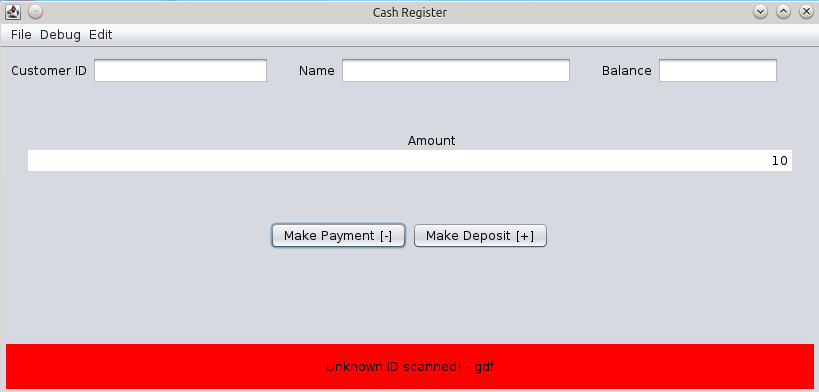
\includegraphics[height=5cm,keepaspectratio]{snapshot4.png}
\captionof{figure}{Unbekannte Tag-ID}
\label{snapshot4}
\end{center}
~\newline
In der Menü-Leiste kann unter \textit{File} die Verbindung gestartet, getrennt
und überprüft werden. \textit{Debug} gibt die Möglichkeit eine Tag-ID
einzugeben, um so die Funktionsfähigkeit des Programms zu kontrollieren, ohne einen echten
Reader anschließend zu müssen.
\newline
\textit{ACHTUNG: Dies ist momentan nicht funktionsfähig, da das Programm auf
die Nutzung im Praktikum spezialisiert wurde.}
\newline
Unter \textit{Edit} können die in Abbildung \ref{snapshot5} gezeigen
Einstellungen abgerufen und geändert werden.
\begin{center}
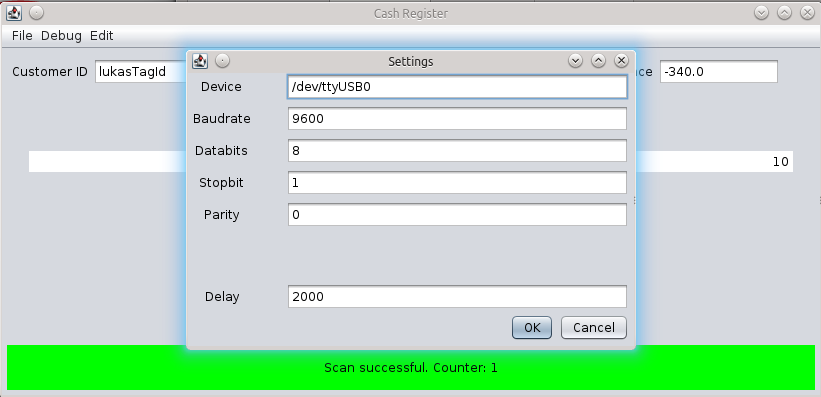
\includegraphics[height=5cm,keepaspectratio]{snapshot5.png}
\captionof{figure}{Settings}
\label{snapshot5}
\end{center}
Hier sind alle Einstellungen der seriellen Schnittstelle vorzunehmen.
~\newline
\section{Beschreibung der Realisierung mittels UML Klassendiagrammen}
Das Programm ist nach dem Paradigma des Model-View-Controller Patterns aufgebaut. Die meisten Klassen des Controllers und der View sind als Singletonpattern realisert. Daher erfolt die Referenzübergabe über den Aufruf getInstance() der jeweiligen Klasse. Das Model braucht als Einzige Zugriff auf die Datenbank und ist daher von SQLConnection abgeleitet.

\section{Anhang}
\begin{figure}[htb] \centering
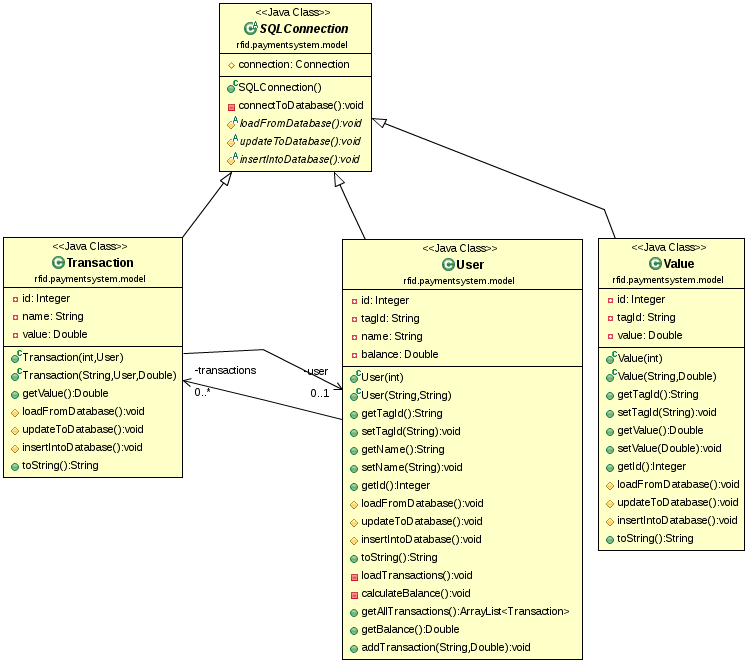
\includegraphics[width=\textwidth,keepaspectratio=true]{UML_Model.png}
\caption{MVC - Model}
\end{figure}
\begin{figure}[htb] \centering
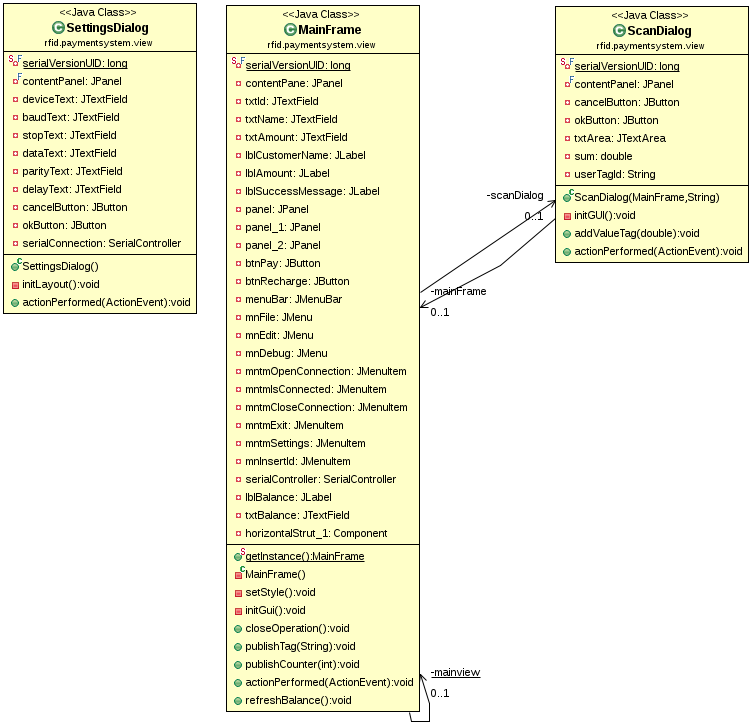
\includegraphics[width=\textwidth,keepaspectratio=true]{UML_View.png}
\caption{MVC - View}
\end{figure}
\begin{figure}[htb] \centering
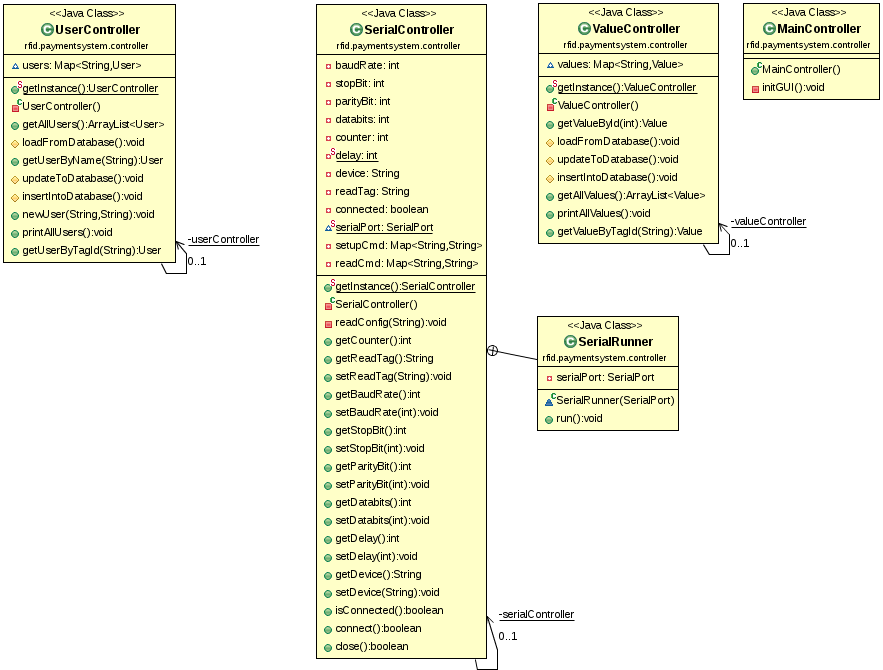
\includegraphics[width=\textwidth,keepaspectratio=true]{UML_Controller.png}
\caption{MVC - Controller}
\end{figure}

\end{document}
